% The diagram in examples/tikz-demo.tex. Compile with pdflatex, then make the PNG the editor
% shows: pdftoppm -png -r 200 -singlefile pipeline.pdf pipeline
\documentclass[tikz,border=6pt]{standalone}
\usetikzlibrary{positioning,arrows.meta}
\begin{document}
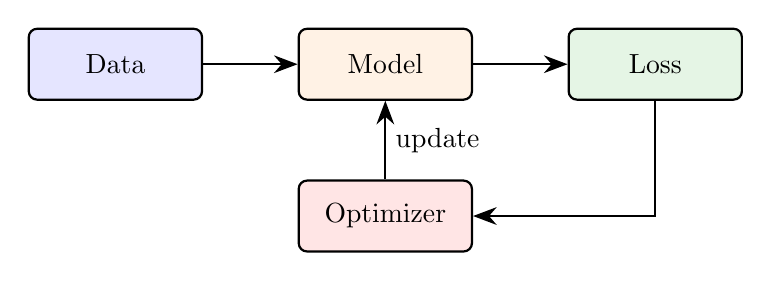
\begin{tikzpicture}[
    box/.style={draw, rounded corners=3pt, thick, minimum height=9mm, minimum width=22mm, fill=#1!10},
    box/.default=gray,
    >={Stealth[length=3mm]}
  ]
  \node[box=blue] (data) {Data};
  \node[box=orange, right=12mm of data] (model) {Model};
  \node[box=green!60!black, right=12mm of model] (loss) {Loss};
  \node[box=red, below=10mm of model] (opt) {Optimizer};
  \draw[->, thick] (data) -- (model);
  \draw[->, thick] (model) -- (loss);
  \draw[->, thick] (loss) |- (opt);
  \draw[->, thick] (opt) -- node[right] {update} (model);
\end{tikzpicture}
\end{document}
